\section{排版图片}

\subsection{支持图片格式}

模板支持的图片格式有:jpg,pdf,eps,png等。既然选择了 \LaTeX,那就尽量使用pdf,eps等矢量图。

\subsection{插入图片方法}

论文中图是很重要的,俗语曰:“一图胜千言,有图有真相”,总之,有图,言者能言之凿凿,观者能察之切切。

\begin{figure}[htbp]
    \centering
    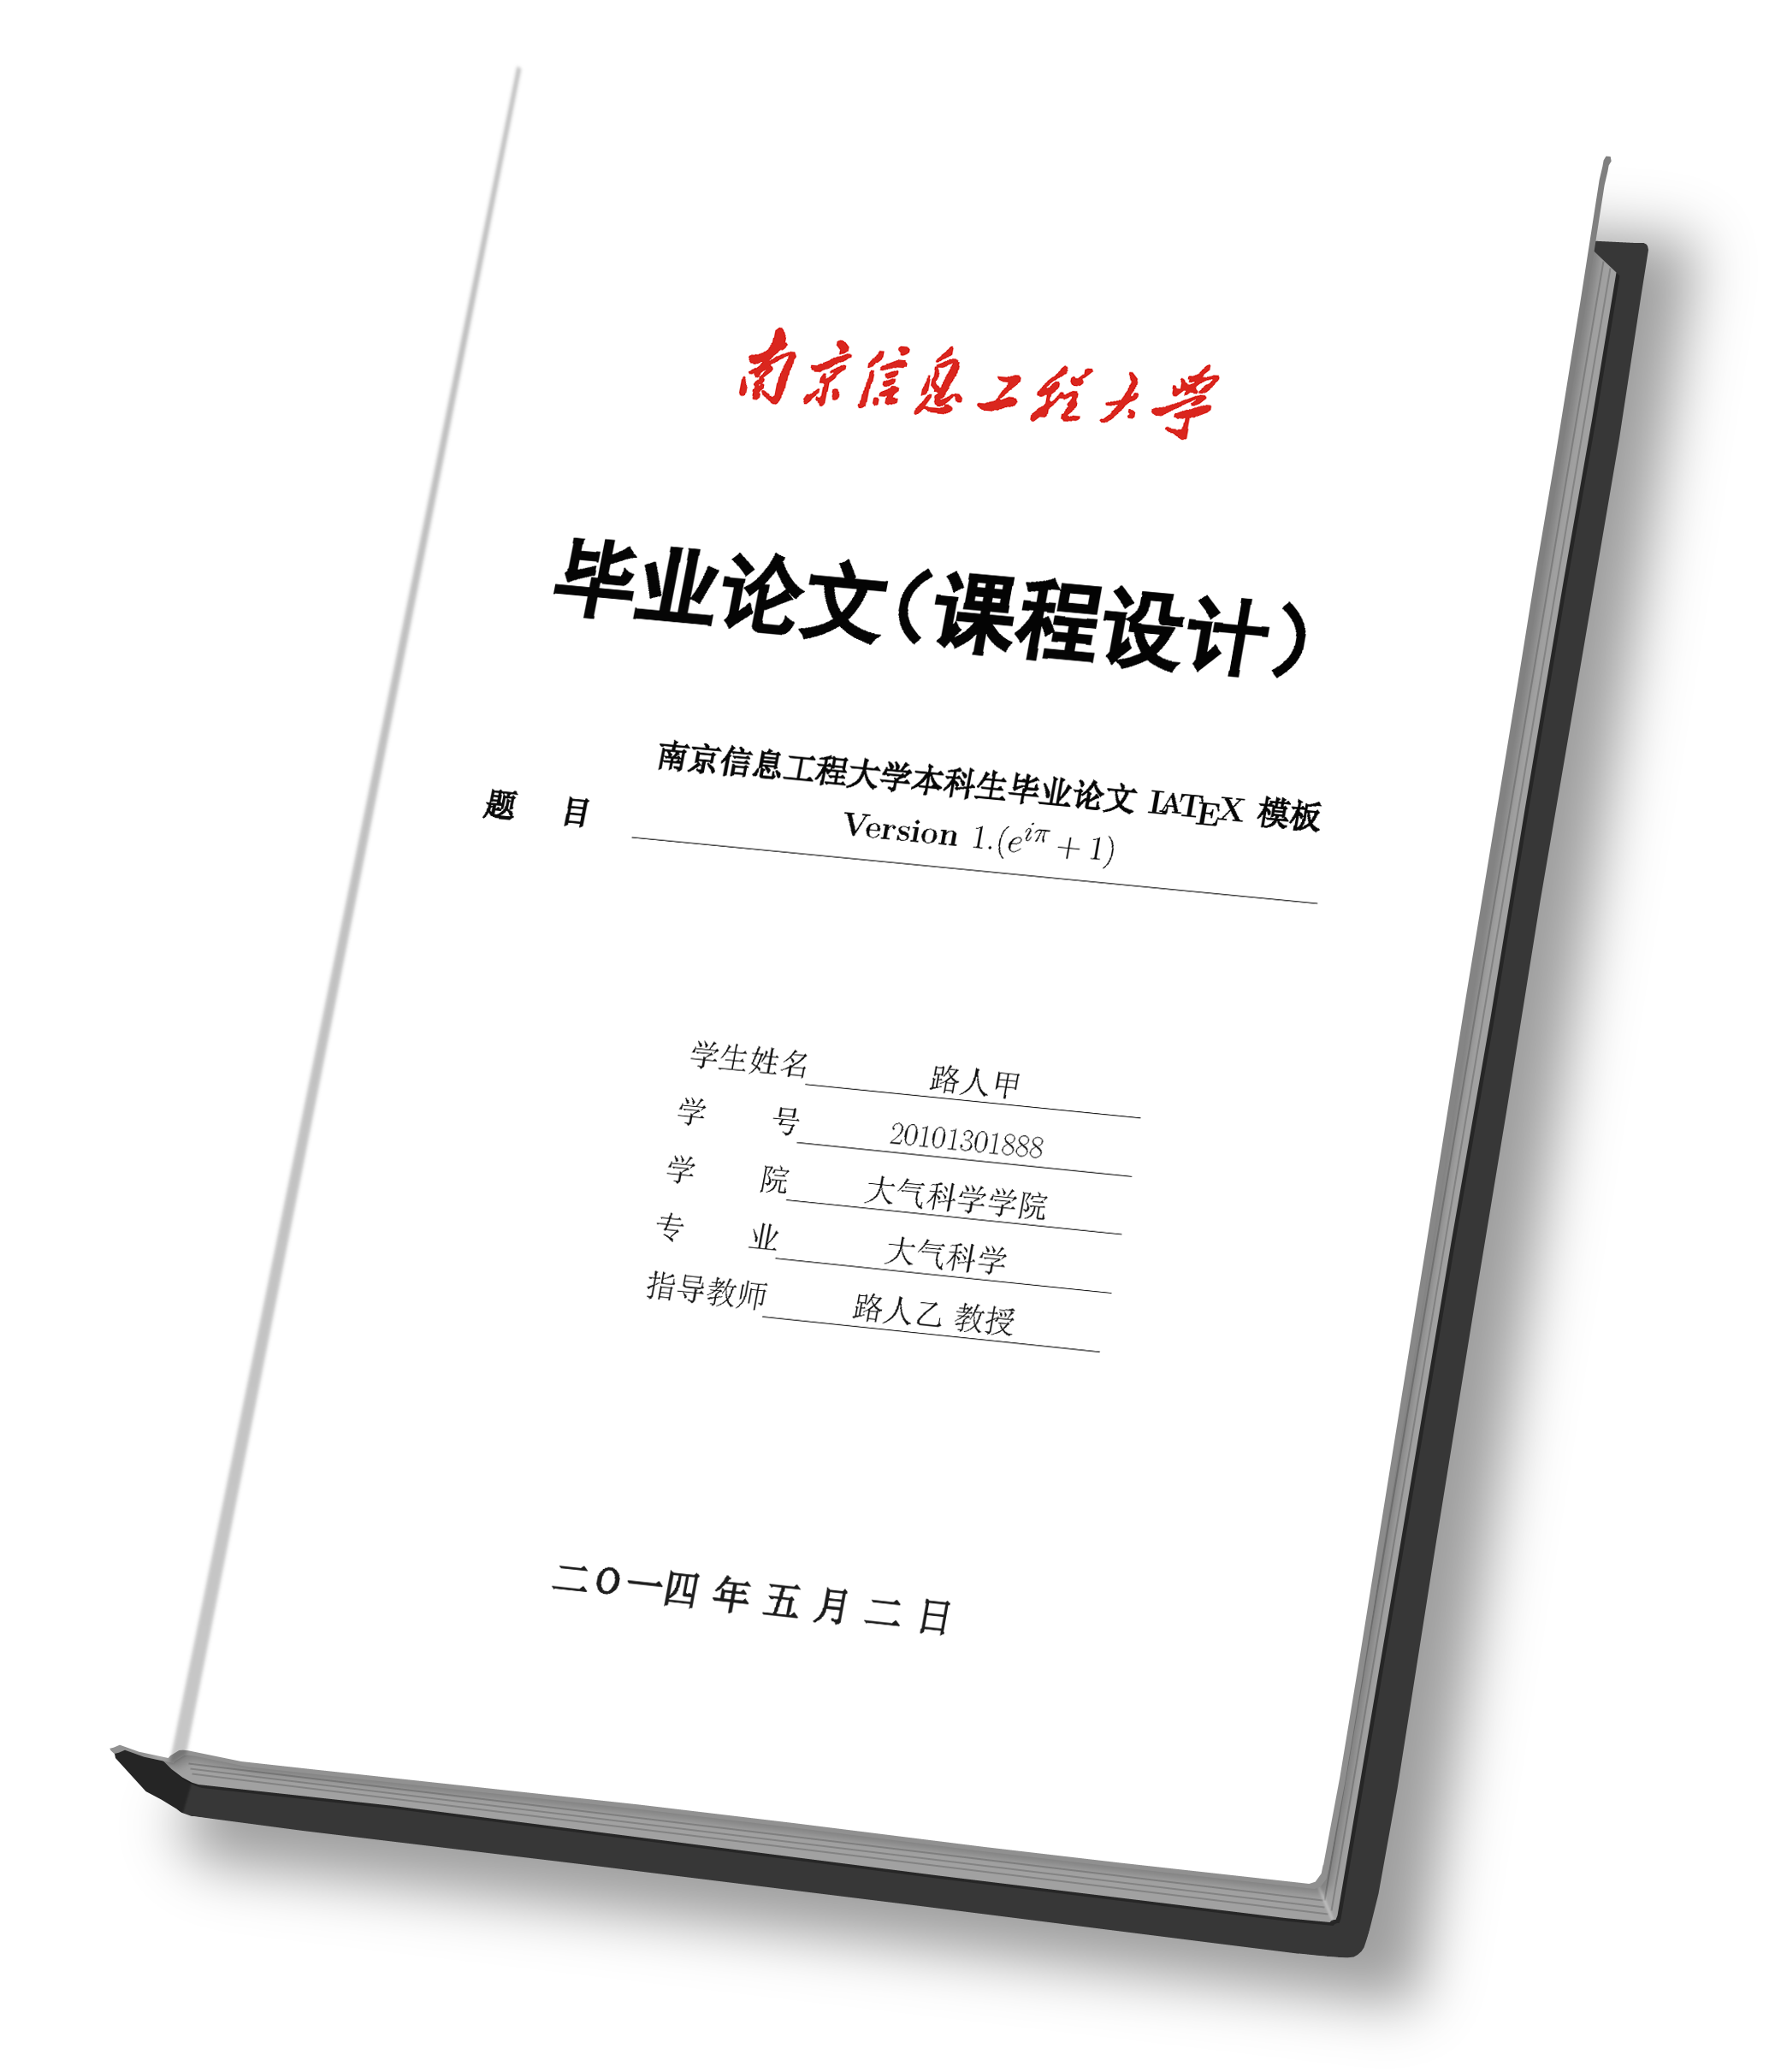
\includegraphics[width=0.6\textwidth]{figs/color/face.png}
    \caption{南京信息工程大学本科生毕业论文\LaTeX 模板封面展示}
    \label{nuist_face}
\end{figure}

图~\ref{nuist_face}~就是插入到文档中的图片,下面展示一下操作的代码:

{\color{green!50!black}
\begin{lstlisting}[breaklines=true,]
\begin{figure}[htbp]
    \centering
    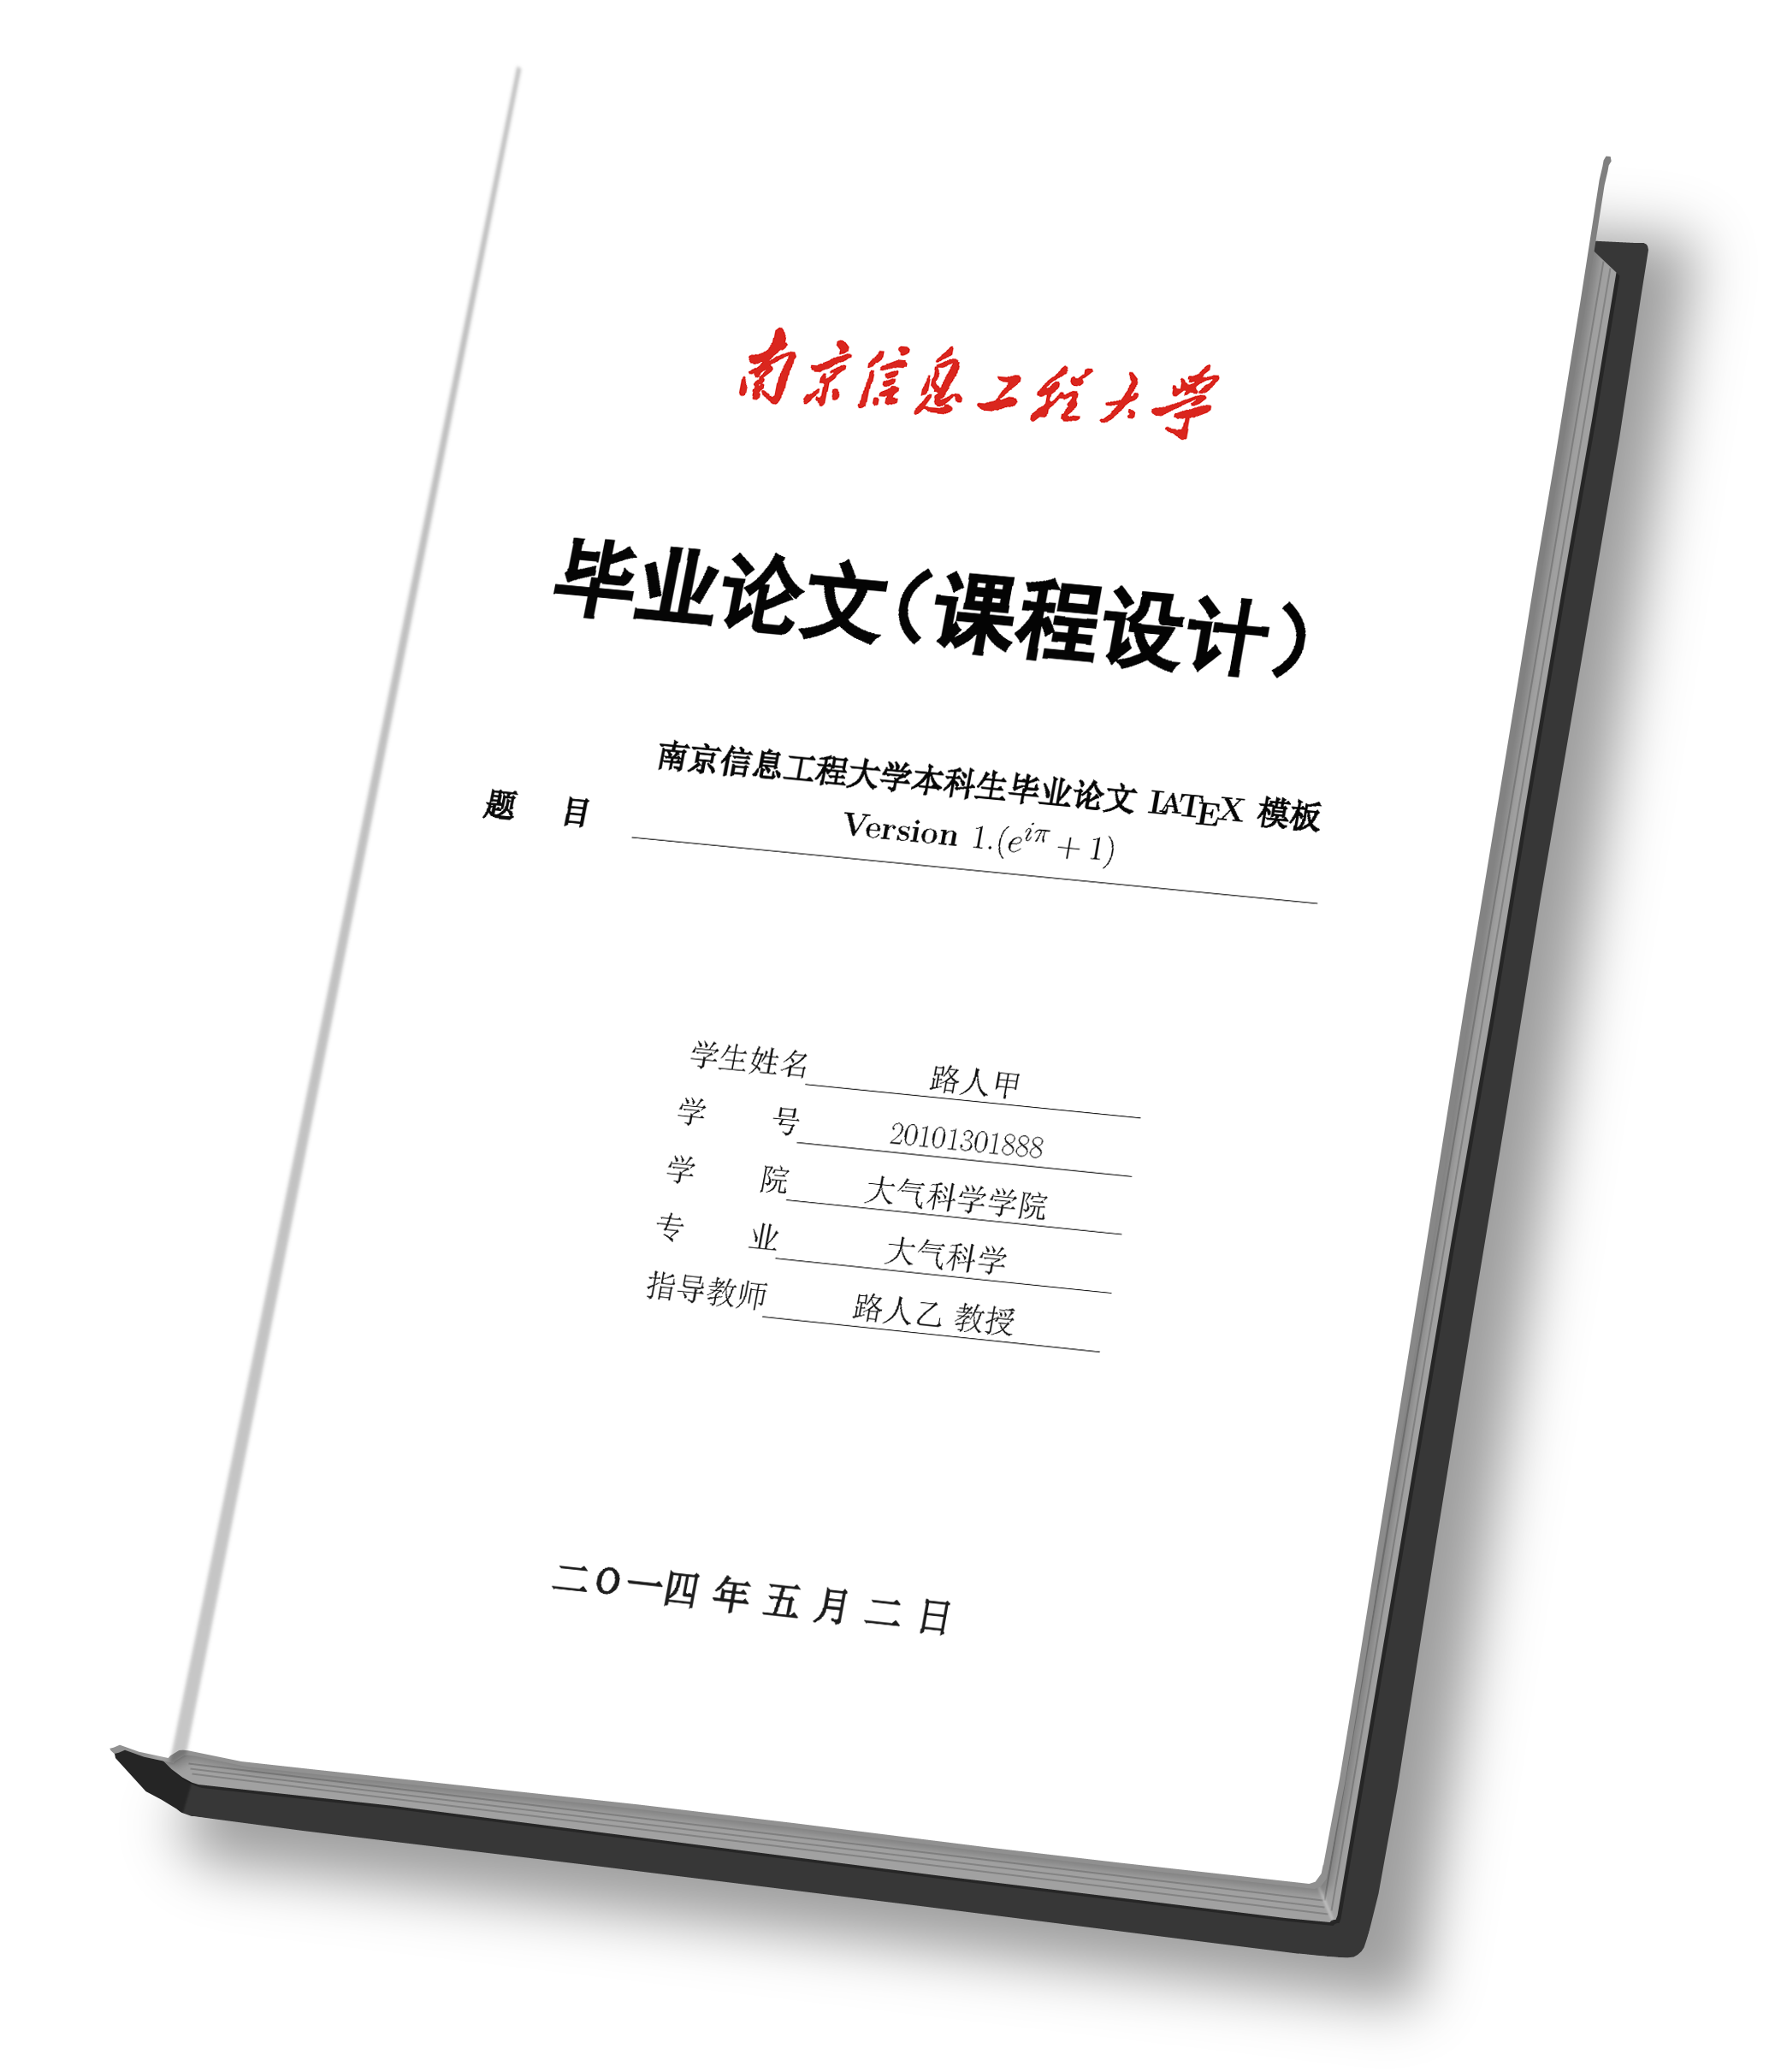
\includegraphics[width=0.6\textwidth]{figs/color/face.png}
    \caption{南京信息工程大学本科生毕业论文\LaTeX 模板封面展示}
    \label{nuist_face}
\end{figure}
\end{lstlisting}
}

\subsection{并列图及添加子图标题}

大家在做论文时的时候经常需要两幅图并排的情况,下面来看看\LaTeX 是怎样精确控制并排图片占位大小的,从而使其各占一半水平空间。如图~\ref{cn_map}~:

\begin{figure}[htbp!]
    \centering
    \includegraphics[width=0.5\textwidth]{figs/color/china1.png}\includegraphics[width=0.5\textwidth]{figs/color/china2.png}
    \caption{中国地图展示(左图为素颜,右图为彩妆)}
    \label{cn_map}
\end{figure}

其实现代码如下:

{
\color{green!50!black}
\begin{lstlisting}[breaklines=true,]
\begin{figure}[htbp!]
    \centering
    \includegraphics[width=0.5\textwidth]{figs/color/china1.png}\includegraphics[width=0.5\textwidth]{figs/color/china2.png}
    \caption{中国地图展示(左图为素颜,右图为彩妆)}
    \label{cn_map}
\end{figure}
\end{lstlisting}
}

是不是感觉图~\ref{cn_map}~的标题不太专业,也想给左右两个子图各加一个标题?那其实也很简单,模板引入了subfigure宏包实现。实现后效果如图~\ref{subfig_cn_map}~:

\begin{figure}[htbp!]
    \centering
    \subfigure[素颜\label{fig:sub1}]{\includegraphics[width=0.5\textwidth]{china1.png}}
    \subfigure[彩妆\label{fig:sub2}]{\includegraphics[width=0.5\textwidth]{china2.png}}
    \caption{中国地图展示}
    \label{subfig_cn_map}
\end{figure}

当然我们在引用的时候,可以引用母图,如图~\ref{subfig_cn_map}~,也可以引用子图,如图~\ref{subfig_cn_map}\subref{fig:sub1}~,图~\ref{subfig_cn_map}\subref{fig:sub2}~。

好了让我们来看实现的代码吧:

{
\color{green!50!black}
\begin{lstlisting}[breaklines=true,]
\begin{figure}[htbp!]
    \centering
    \subfigure[素颜\label{fig:sub1}]{\includegraphics[width=0.5\textwidth]{china1.png}}
    \subfigure[彩妆\label{fig:sub2}]{\includegraphics[width=0.5\textwidth]{china2.png}}
    \caption{中国地图展示}
    \label{subfig_cn_map}
\end{figure}
\end{lstlisting}
}

最后再给出一个例子,例如大家在做EOF分析时,可能要两个模态之间进行对比,我们知道每一个模态场都有一个时间序列与其对应,所以这样我们还可能用到$2\times 2$形式的图片排列方式,如图~\ref{fig:eof_12}~。

\begin{figure}[htbp]
    \center
    \subfigure[第一模态]{\label{eof_1}
        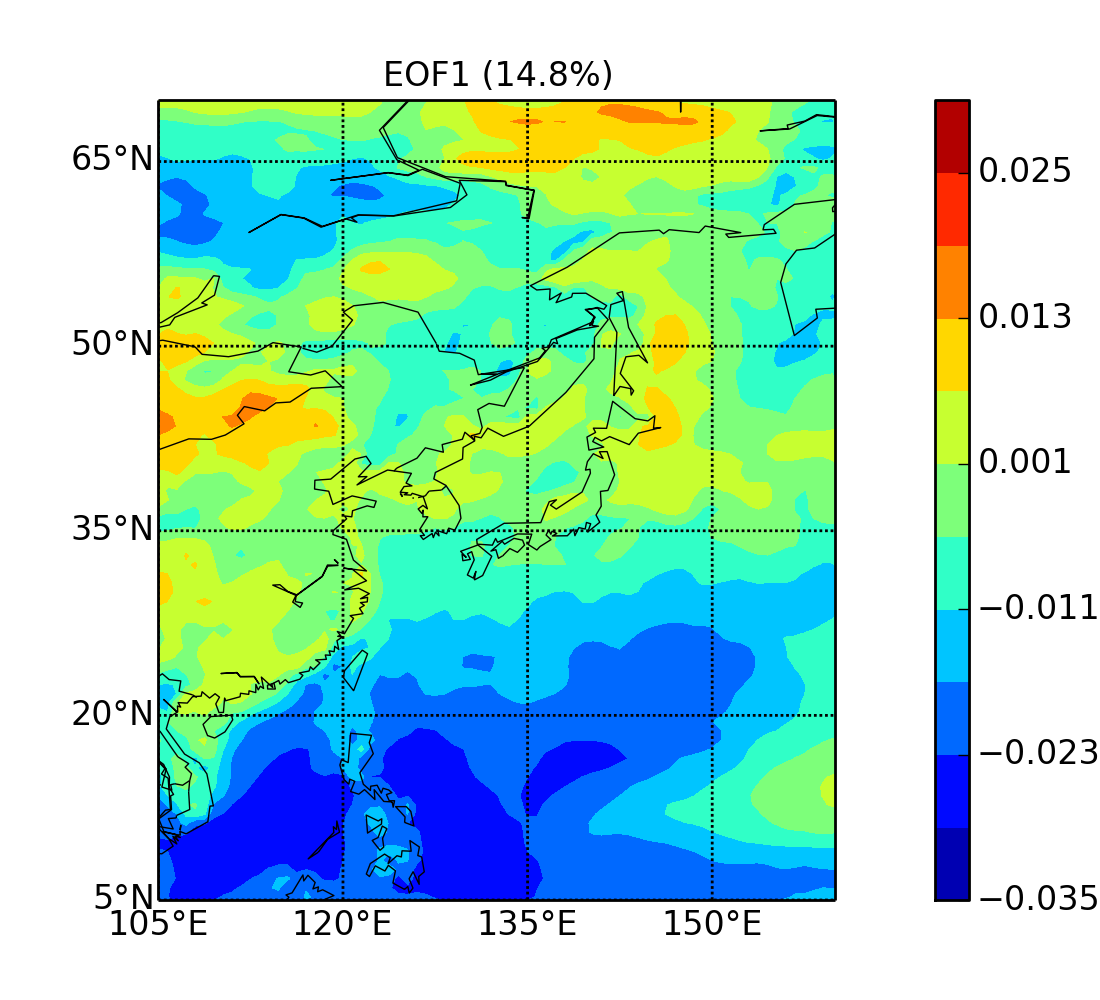
\includegraphics[width=0.4\textwidth]{eof1.png}
    }
    \subfigure[第二模态]{\label{eof_2}
        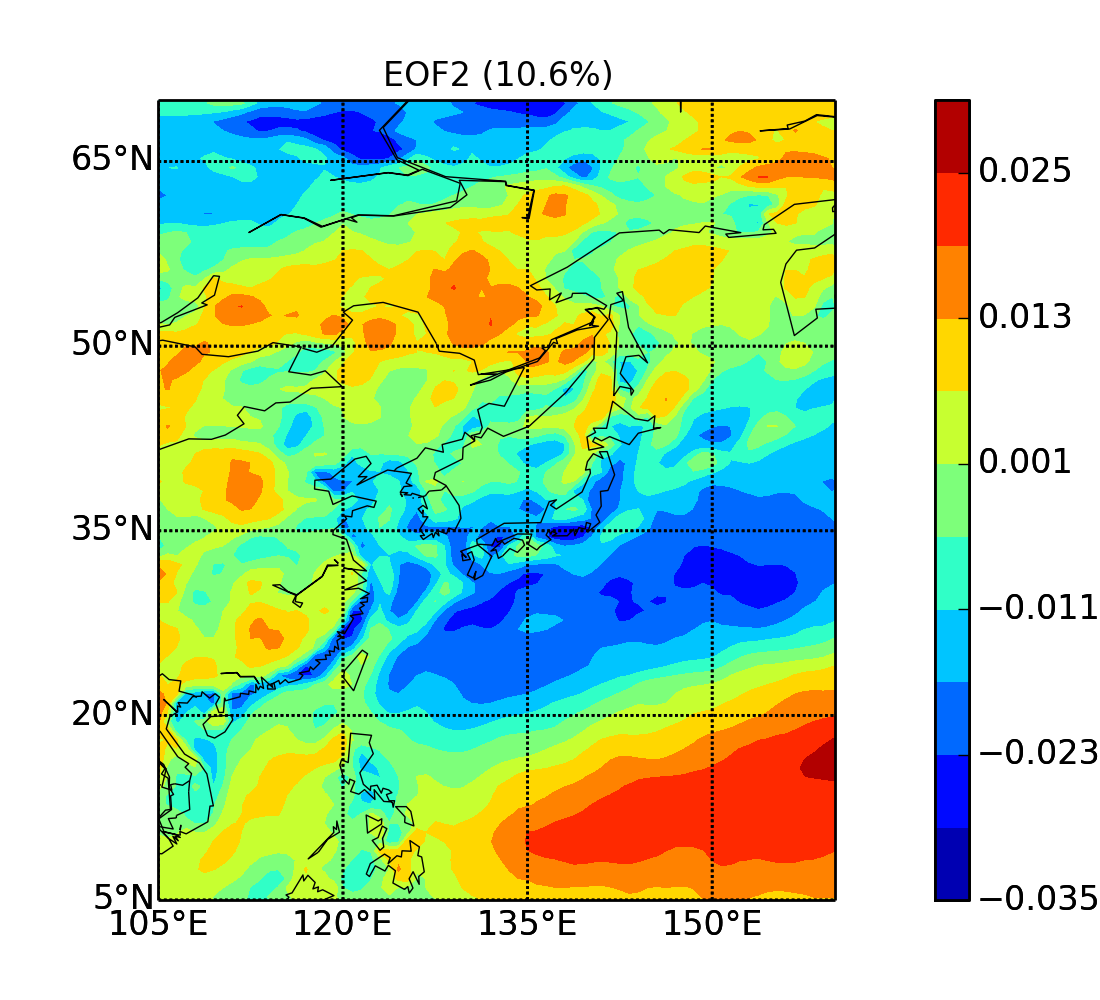
\includegraphics[width=0.4\textwidth]{eof2.png}
    }
    \\
    \subfigure[第一模态对应的时间系数]{\label{eof_t1}
        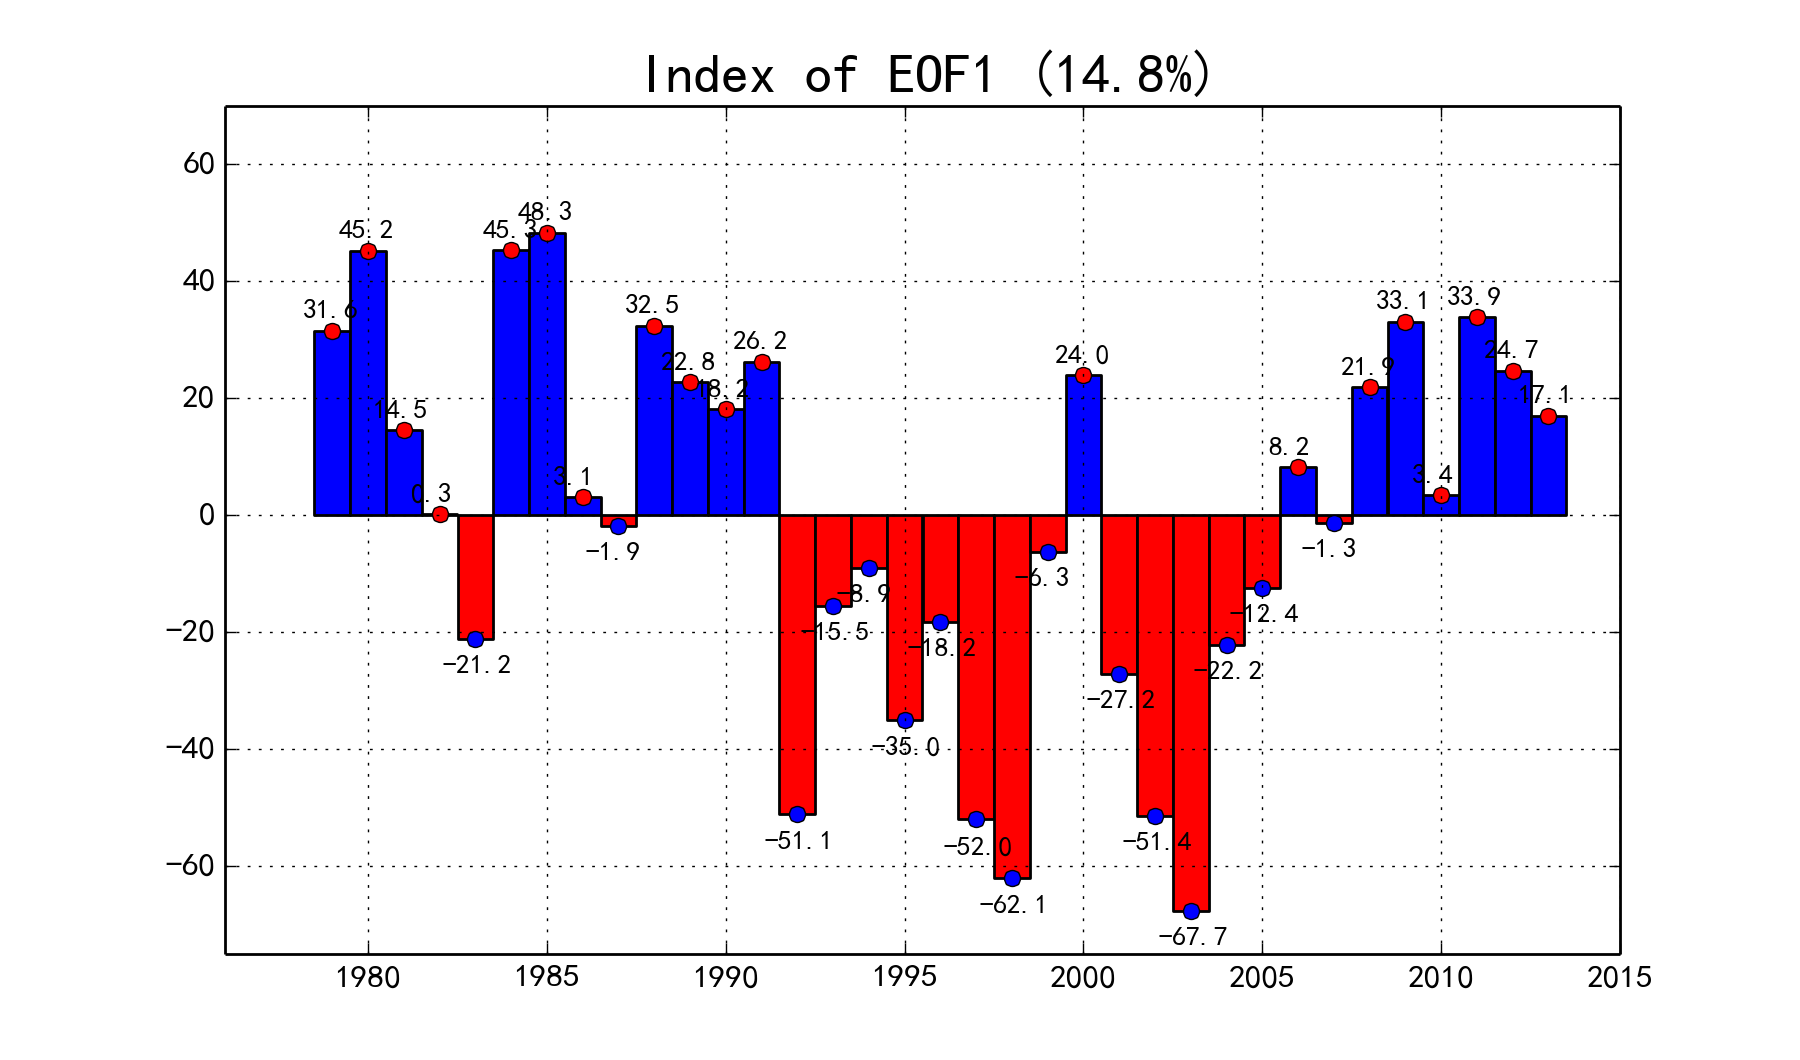
\includegraphics[width=0.4\textwidth]{t1.png}
    }
    \subfigure[第二模态对应的时间系数]{\label{eof_t2}
        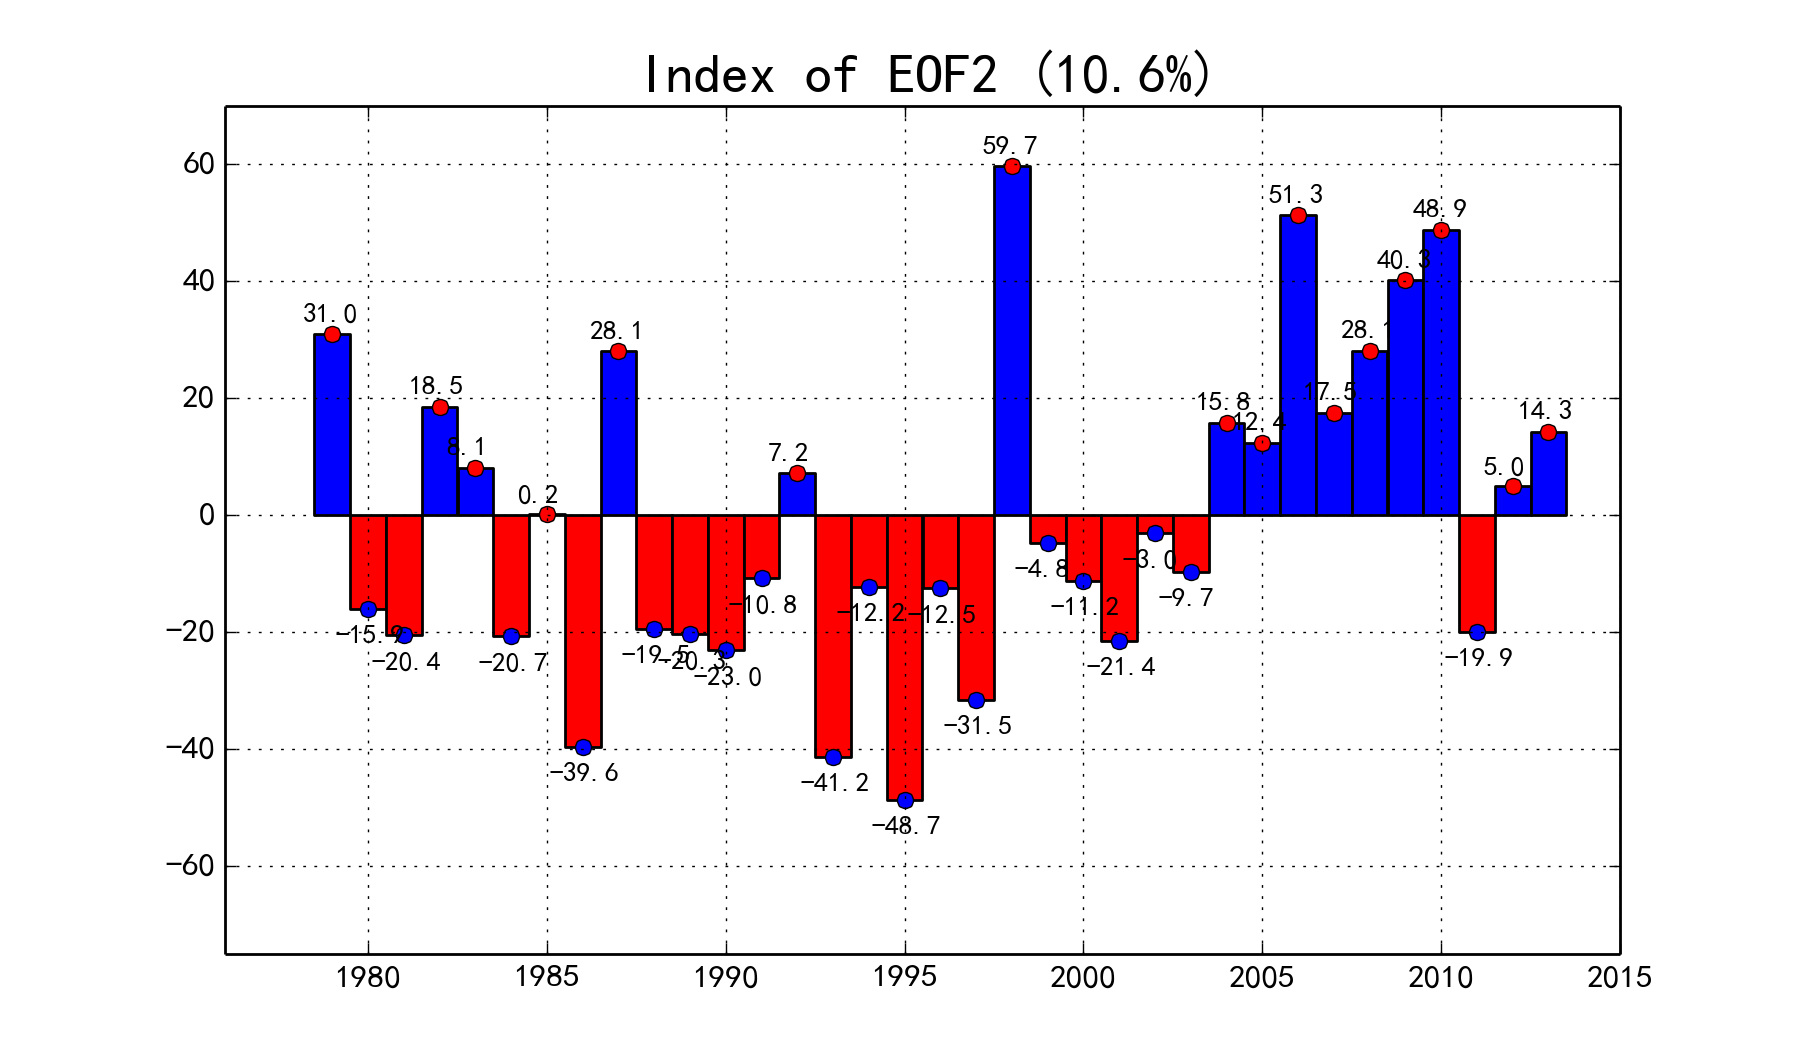
\includegraphics[width=0.4\textwidth]{t2.png}
    }
    \caption{ABLH的EOF分析结果(第一第二模态及其时间系数)}\label{fig:eof_12}
\end{figure}

我们可以用下面的命令来实现:

{
\color{green!50!black}
\begin{lstlisting}[breaklines=true,]
\begin{figure}[htbp]
    \center
    \subfigure[第一模态]{\label{eof_1}
        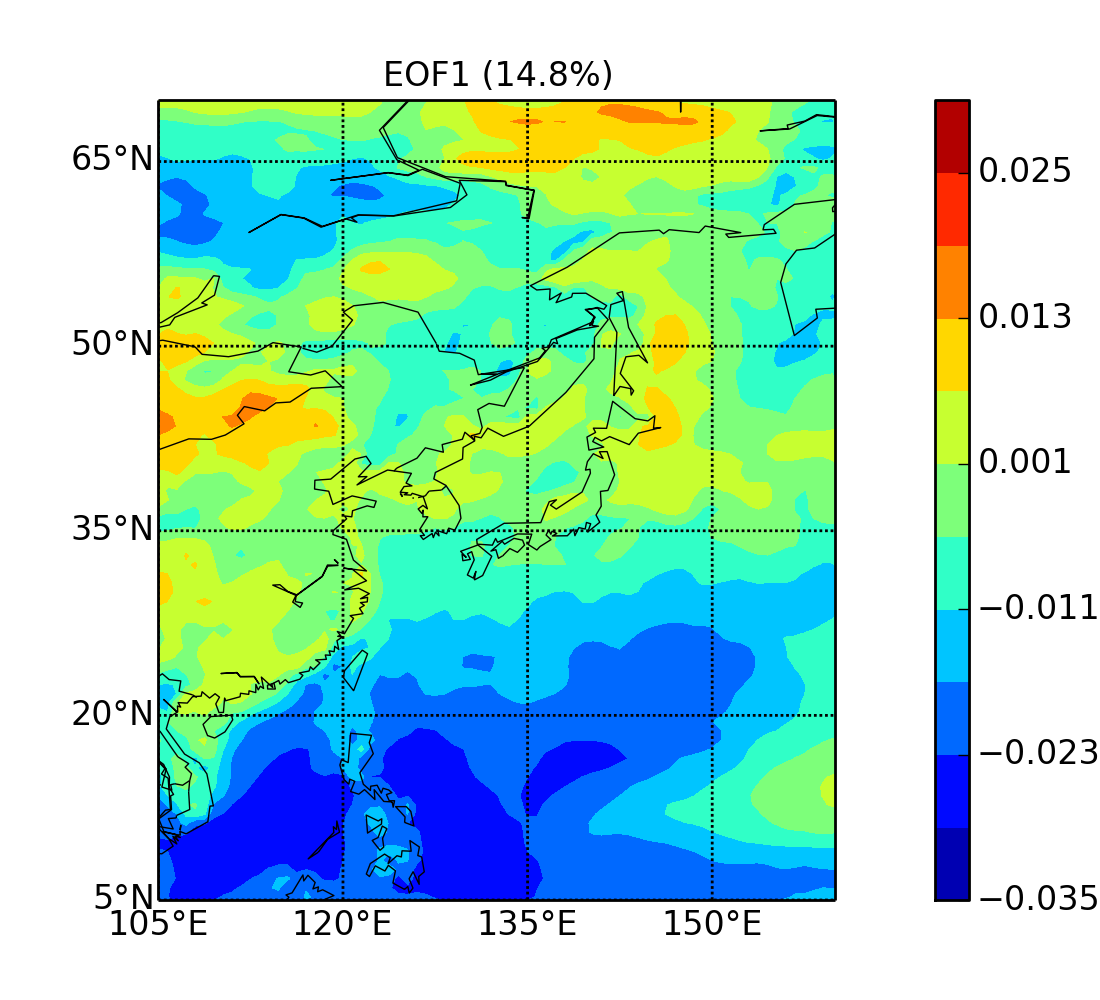
\includegraphics[width=0.4\textwidth]{eof1.png}
    }\subfigure[第二模态]{\label{eof_2}
        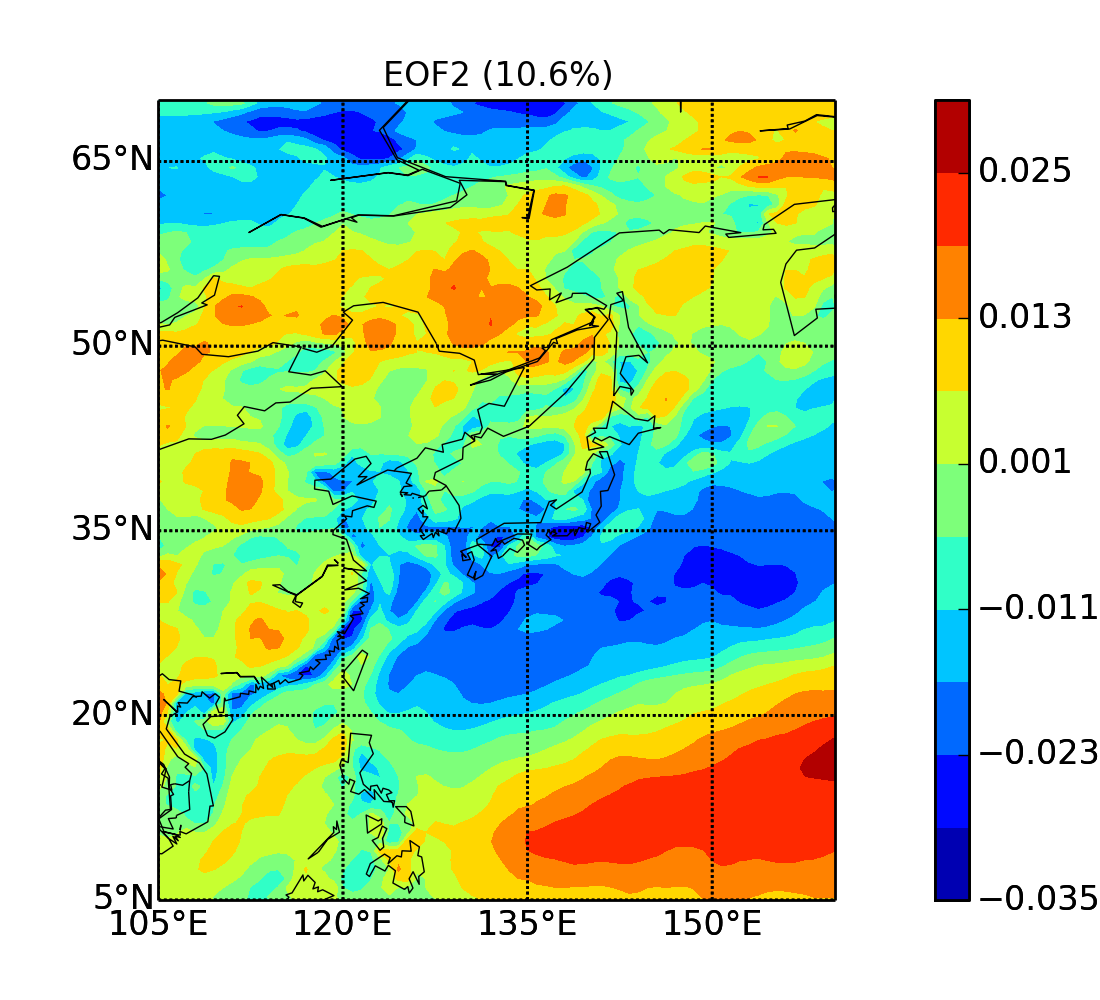
\includegraphics[width=0.4\textwidth]{eof2.png}
    }
    \\
    \subfigure[第一模态对应的时间系数]{\label{eof_t1}
        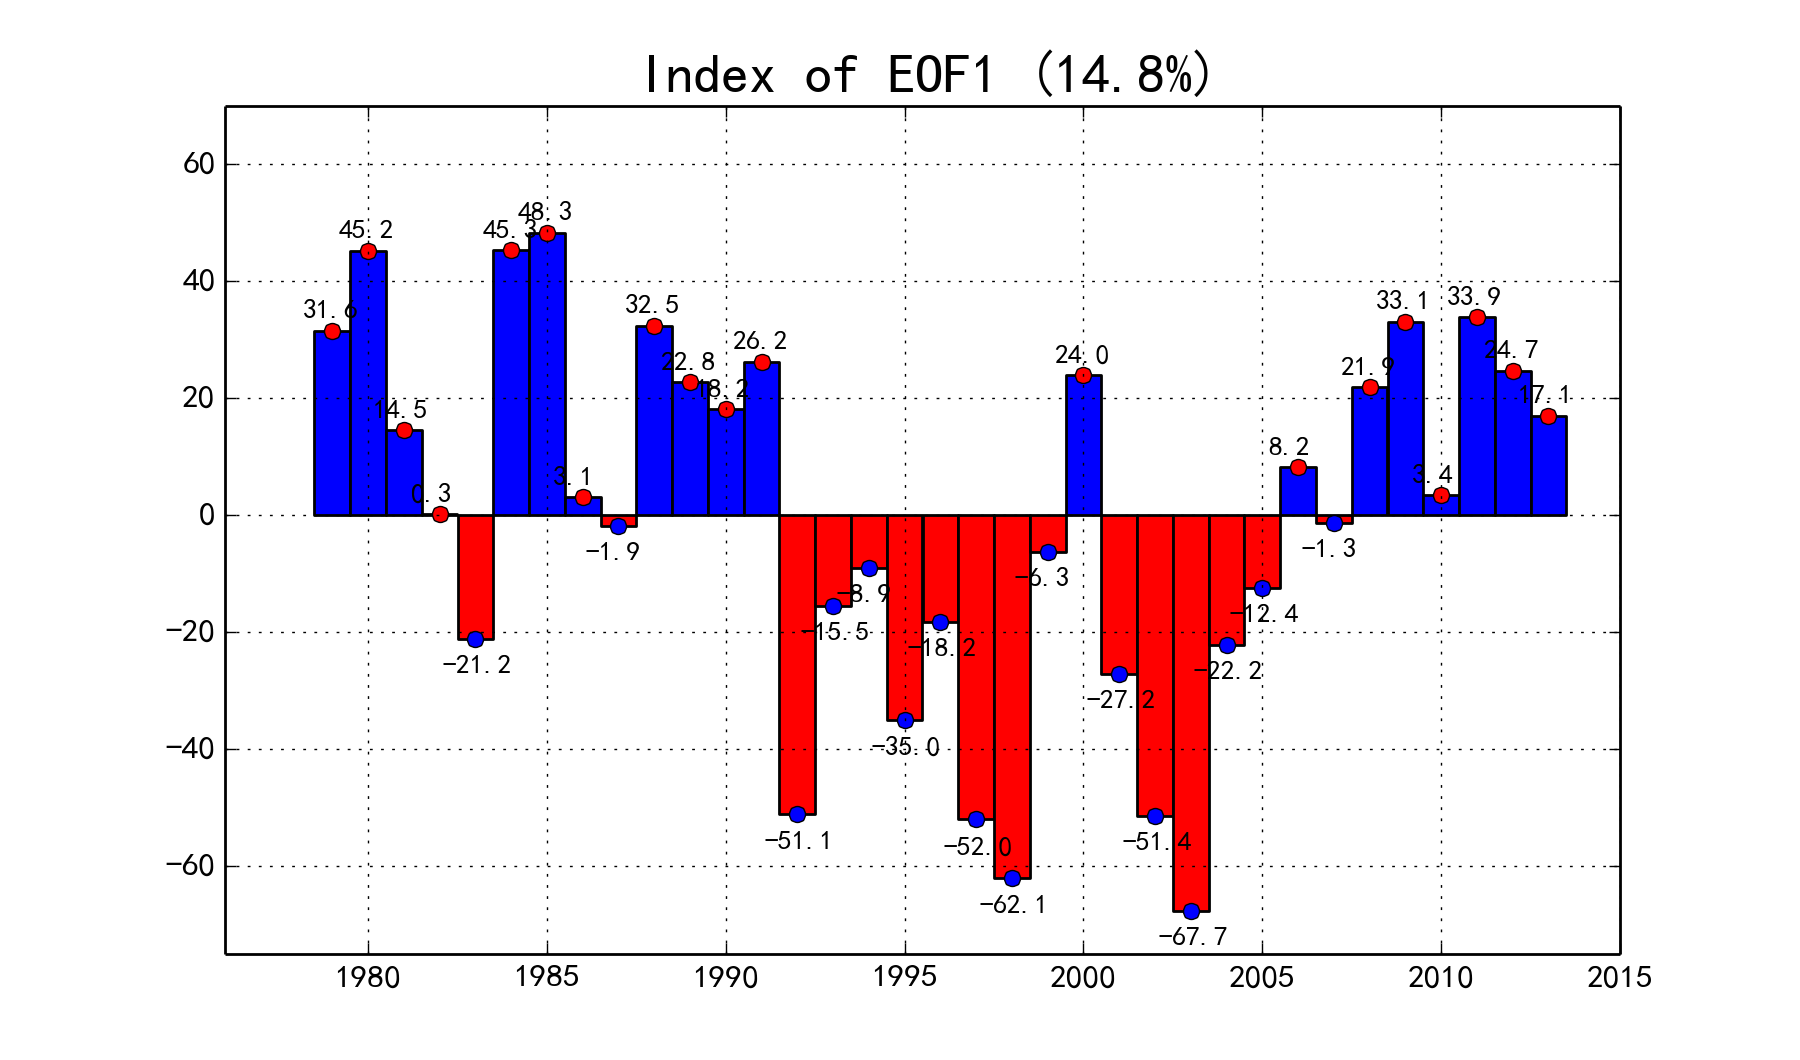
\includegraphics[width=0.4\textwidth]{t1.png}
    }\subfigure[第二模态对应的时间系数]{\label{eof_t2}
        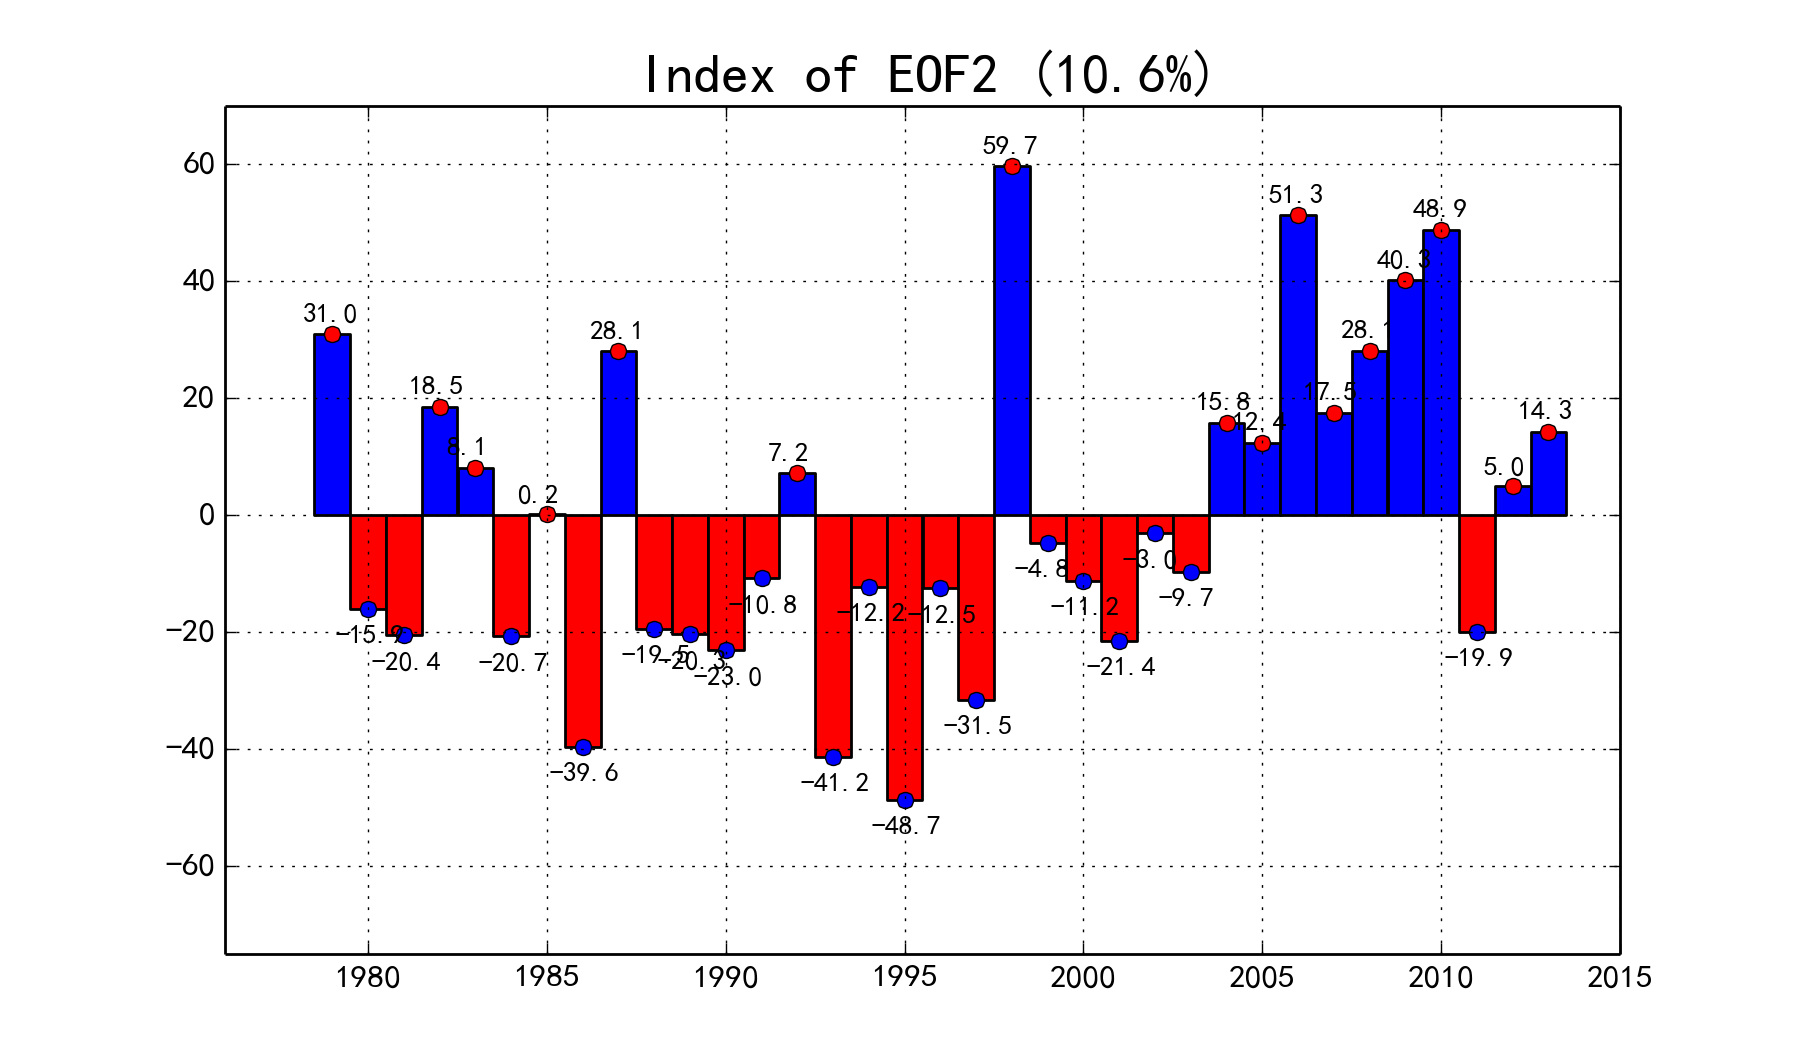
\includegraphics[width=0.4\textwidth]{t2.png}
    }
    \caption{ABLH的EOF分析结果(第一第二模态及其时间系数)}\label{fig:eof_12}
\end{figure}
\end{lstlisting}
}

朋友们应该也发现奥秘所在了,对,就是那个双斜线 $\backslash\backslash$ 的作用,双斜线在\LaTeX 排版系统中就是换行的命令,知道了这一点,大家可以随意安排自己的图片了,可以用$2\times 3$或者$3\times 2$来摆放自己插图了。

\subsection{图片文件夹的指定}

细心的朋友可能会发现生成~\ref{subfig_cn_map}~和图~\ref{cn_map}~所用的代码在指定图片路径时的写法不同,一种是相对路径,另一种是只有图片名称。这是为什么呢?原因很简单。为了在写作时引用图片方便,本文在导言区写上这样的\verb|\graphicspath{{figs/color/}}|一名命令,来宏观地指定图片所存放的位置。

这一功能的好处就是,对于有的同学电子文档和打印文档所用图片色彩格式不同,这样只要一条命令就可以切换到另一个文件夹了,比较实用。
